\documentclass[journal]{IEEEtran}
% Layout follows IEEE Access (two-column journal). For submission, move the body into the official
% ieeeaccess.cls template from ieeeaccess.ieee.org; section structure and references carry over unchanged.
% Every number below is inserted by `python -m sieve paper` from the run logs (placeholders «...»).
\usepackage{amsmath,amssymb}
\usepackage{newtxtext,newtxmath}
\usepackage{graphicx}
\usepackage{booktabs}
\usepackage{multirow}
\usepackage{xcolor}
\usepackage{url}
\usepackage{algorithm}
\usepackage{algpseudocode}
\usepackage{tikz}
\usetikzlibrary{positioning,arrows.meta,fit,backgrounds,calc}
\usepackage{cite}
\usepackage{pifont}
\newcommand{\cmark}{\ding{51}}
\newcommand{\xmark}{\ding{55}}
\newcommand{\pmark}{$\circ$}
\definecolor{accessblue}{RGB}{0,98,155}
\definecolor{lanegold}{RGB}{255,214,10}
\makeatletter
\def\ps@accesshead{\def\@oddhead{\footnotesize\color{accessblue}\textsf{IEEE Access}\hfill\textsf{Preprint --- not peer reviewed}}\def\@evenhead{\@oddhead}%
\def\@oddfoot{\hfil\footnotesize\thepage\hfil}\def\@evenfoot{\@oddfoot}}
\makeatother
\begin{document}
\title{Sieve: Cache-Aware, Segment-Level Routing Across Compression, KV-Prefix Reuse and Externalization for Local Large Language Model Prompts}
\author{\IEEEauthorblockN{[Author Name]\IEEEauthorrefmark{1}}\\
\IEEEauthorblockA{\IEEEauthorrefmark{1}[Department], [Institution], [City, Country]}\\
Corresponding author: [Author Name] (e-mail: [address]).}
\markboth{IEEE Access}{Sieve: Segment-Level Prompt Routing for Local LLMs}
\maketitle
\pagestyle{accesshead}\thispagestyle{accesshead}

\begin{abstract}
Local large language models share one fixed context window between the prompt and the answer, and long conversations waste it on verbose, repeated and stale text. Prompt compression reduces tokens but rewrites the prefix, which defeats the key-value (KV) prefix cache that local servers rely on. This paper presents Sieve, a middleware that splits each request into segments and routes every segment to one of three lanes: COMPRESS (LLMLingua-2 pruning at a per-segment ratio, checked by a rule-based verifier of facts and their context), CACHE (kept byte-identical so the KV prefix is reused) or EXTERNALIZE (replaced by a deterministic stub that the model can expand through a tool call). Hard rules run first, a cost-sensitive gradient-boosting classifier routes the rest, and a per-session ledger replays emitted strings so compression does not invalidate the cached prefix. On 180 ground-truth questions from 76 synthetic conversations with invented entities, run on Qwen3-14B through Ollama with a 4096-token window, Sieve reduced prompt tokens by 31.0\% (95\% CI 27.8--34.0\%) and raised mean output headroom from 1,349 to 2,393 tokens. Its accuracy change of +5.0 percentage points (CI -0.6 to +11.1) is not statistically distinguishable from zero, while on prompts that overflowed the window accuracy rose by 36.2 points (CI +19.1 to +53.2). Median time to first token on cold questions fell by 1.12 s. A controlled test shows that re-compressing a prefix reduces prefill reuse from 95\% to 2\%, and that sending the memoized compressed string restores it to 89\%. Code, logs and traces are public.
\end{abstract}

\begin{IEEEkeywords}
Large language models, prompt compression, key-value cache, context management, local inference, cost-sensitive classification, retrieval on demand.
\end{IEEEkeywords}

%=====================================================================
\section{Introduction}
\IEEEPARstart{L}{arge} language models (LLMs) are increasingly run on local hardware for privacy, cost and latency
reasons~\cite{qu2025edge,schwartz2020green}. A local deployment exposes one hard resource: the context window, here
$n_\text{ctx}=4096$ tokens, shared by the system prompt, the conversation history, pasted documents and tool output, and the
answer itself~\cite{naveed2025overview,raiaan2024review}. Long sessions fill it in three distinct ways. Some text is needed but
verbose; some is static and resent on every turn; and some is bulky but rarely relevant, such as an old document or a large tool
dump, a pattern that is common when LLMs are embedded in engineering workflows~\cite{hou2024llm4se}. When the raw prompt exceeds
the window the server silently truncates it, and facts disappear.

Each kind of waste has a known remedy, but the remedies interfere. Token-level prompt compression, for example
Selective Context~\cite{li2023selective}, LLMLingua~\cite{jiang2023llmlingua}, LongLLMLingua~\cite{jiang2024longllmlingua} and
LLMLingua-2~\cite{pan2024llmlingua2}, shortens verbose text. Key-value (KV) prefix caching, as in
PagedAttention~\cite{kwon2023vllm}, Prompt Cache~\cite{gim2024promptcache} and SGLang~\cite{zheng2024sglang}, makes static
prefixes nearly free to re-process. Retrieval on demand, as in memory-managed agents~\cite{packer2023memgpt,zhang2025memory} and
tool-using models~\cite{schick2023toolformer,qin2024tool}, keeps rarely needed text out of the prompt. However, compression
rewrites the prompt, and any change early in the prompt forces the server to prefill every later token again. A compressor that
is re-run on every turn can therefore make warm turns slower even as it makes prompts shorter.

This paper studies whether a \emph{per-segment} routing policy that chooses among compression, caching and externalization,
combined with a mechanism that keeps emitted text byte-stable across turns, reduces prompt tokens and increases output headroom
without losing accuracy. The contributions are:
\begin{itemize}
\item \textbf{Sieve}, a three-lane middleware (COMPRESS, CACHE, EXTERNALIZE) with a rule layer, a cost-sensitive
gradient-boosting router, a fact verifier that checks both atoms and the relation words around them, a session store with
deterministic stubs and an \texttt{expand\_context} tool, and a prefix ledger with budget-driven epochs (Section~\ref{sec:method}).
\item A formulation of budget-constrained lane assignment as a multiple-choice knapsack problem, with a greedy priority allocator
and a complexity analysis of every pipeline stage.
\item A \textbf{controlled measurement of the cache--compression conflict} on a production local server, including a
timing-based estimator of prefix reuse for servers whose token counters do not reveal cache hits.
\item A matched-budget benchmark of seven conditions and five ablations on 180 ground-truth questions, with paired bootstrap
statistics, per-call traces and an automatically generated list of supported and unsupported claims. Code, logs and traces are
public~\cite{sieve2026code}.
\end{itemize}
Section~\ref{sec:related} reviews related work, Section~\ref{sec:method} presents Sieve, Section~\ref{sec:exp} describes the
experimental methodology, Section~\ref{sec:results} reports the results, Section~\ref{sec:discussion} discusses them and their
limits, and Section~\ref{sec:conclusion} concludes.

%=====================================================================
\section{Related Work}\label{sec:related}
\subsection{Large Language Models and Prompting}
Pre-trained language models evolved from task-specific encoders into general LLMs; surveys trace this
path~\cite{qiu2020ptm,han2021ptm,min2023recent} and the architectures and training regimes of current
LLMs~\cite{naveed2025overview,raiaan2024review,yang2024harnessing,lin2022transformers}. Prompting became the main interface to
these models~\cite{liu2023prompting,chen2025promptengineering}, and evaluation practice has had to follow~\cite{chang2024evaluation}.
We use Qwen3~\cite{qwen3}, an open-weight model family that can be served locally and supports tool calls with or without
explicit reasoning. These works establish that prompt content drives model behaviour. They do not address how to fit a growing
conversation into a fixed window at minimum cost.

\subsection{Efficient Models and Inference}
One line of work lowers the cost per token. Efficient transformer variants change the attention
mechanism~\cite{tay2022efficient,fournier2023practical}, and broader surveys cover efficient methods across the NLP
pipeline~\cite{treviso2023efficient}. Model compression shrinks the network itself through quantization, pruning and
distillation~\cite{zhu2024compression,deng2020compression,cheng2024pruning,gou2021distillation}, which is essential on edge
devices~\cite{qu2025edge} and motivated by the energy cost of large models~\cite{schwartz2020green}. Sieve is complementary: it
leaves the model unchanged and reduces the number of tokens the model must process.

\subsection{Prompt and Context Compression}
Hard-prompt methods delete tokens. Selective Context removes content with low self-information~\cite{li2023selective};
LLMLingua uses a small language model with a budget controller that assigns different ratios to prompt
components~\cite{jiang2023llmlingua}; LongLLMLingua adds question-aware compression and document
reordering~\cite{jiang2024longllmlingua}; LLMLingua-2 casts compression as token classification with a distilled
encoder~\cite{pan2024llmlingua2}; and reinforcement learning has been used to learn discrete edit policies~\cite{jung2024discrete}.
Soft-prompt methods compress into learned vectors (gist tokens~\cite{mu2023gist}, AutoCompressors~\cite{chevalier2023autocompressor})
and therefore require changes to the target model, while RECOMP compresses retrieved documents with trained extractive and
abstractive compressors~\cite{xu2024recomp}. Extractive summarization offers a further family of length-reduction
techniques~\cite{elkassas2021summarization}. All of these apply a single policy to the prompt or to one component of it, and none
accounts for the effect of compression on the server's prefix cache.

\subsection{KV-Cache Reuse and Serving}
Serving systems reuse attention state across requests. PagedAttention manages the KV cache in pages and shares
prefixes~\cite{kwon2023vllm}; Prompt Cache precomputes attention for reusable prompt modules~\cite{gim2024promptcache}; SGLang's
RadixAttention reuses prefixes across calls of structured programs~\cite{zheng2024sglang}; and a recent survey organizes serving
optimizations from algorithms to systems~\cite{miao2025serving}. The llama.cpp engine~\cite{llamacpp} used by Ollama~\cite{ollama}
reuses the longest common prefix with earlier requests. These systems make an unchanged prefix cheap; Sieve shapes prompts so that
the prefix stays unchanged when compression is used.

\subsection{Retrieval, External Memory and Tools}
Retrieval-augmented generation fetches relevant text at query time~\cite{huang2026ragsurvey,zhu2025irsurvey}, typically with dense
retrievers~\cite{zhao2024dense} built on sentence encoders such as Sentence-BERT~\cite{reimers2019sbert} and
MiniLM~\cite{wang2020minilm}. Agent architectures keep long-term memory outside the prompt~\cite{zhang2025memory,wang2024agents,xi2025agents};
MemGPT pages context in and out through function calls~\cite{packer2023memgpt}. Toolformer showed that models can learn when to
call tools~\cite{schick2023toolformer}, and tool learning has since been surveyed broadly~\cite{qin2024tool}. Sieve's EXTERNALIZE
lane is a deterministic, session-scoped instance of this idea, evaluated against cheaper alternatives under one budget.

\subsection{Long Contexts and Faithfulness}
Models do not use long contexts uniformly: information in the middle of the prompt is used less reliably than information at the
ends~\cite{liu2024lost}. Generated answers can also be unfaithful to their input~\cite{ji2023hallucination,huang2025hallucination}.
Both findings shape our design: Sieve keeps chat turns in their original order, checks compressed text for lost facts, and our
benchmark includes needle-position, late-recall and unanswerable questions.

\subsection{Learning and Statistical Methods}
Sieve's router is a gradient-boosting classifier~\cite{friedman2001gbm} with a random-forest ratio regressor~\cite{breiman2001rf},
implemented with scikit-learn~\cite{pedregosa2011sklearn}; class weights address the rarity of the CACHE lane~\cite{he2009imbalanced}.
Results are compared with paired bootstrap intervals~\cite{efron1979bootstrap}, following established advice on comparing learning
systems~\cite{dietterich1998tests}.

\subsection{Research Gap}
Table~\ref{tab:compare} positions Sieve against representative methods. Prior work covers one or two lanes, uses one policy per
prompt or component, and does not control the interaction between compression and prefix caching. Sieve combines all three lanes
under a per-segment policy, verifies compressed facts, and keeps its output byte-stable.
\begin{table}[t]\centering
\caption{Capabilities of representative approaches (\cmark{} yes, \pmark{} partial, \xmark{} no). ``Target unchanged'' means the
served LLM needs no training or modification.}\label{tab:compare}
\setlength{\tabcolsep}{2.2pt}
\resizebox{\columnwidth}{!}{%
\begin{tabular}{lcccccc}\toprule
Approach & Compress & Cache-aware & External. & Per-segment & Target unch. & Fact check\\\midrule
Selective Context~\cite{li2023selective} & \cmark & \xmark & \xmark & \xmark & \cmark & \xmark\\
LLMLingua~\cite{jiang2023llmlingua} & \cmark & \xmark & \xmark & \pmark & \cmark & \xmark\\
LongLLMLingua~\cite{jiang2024longllmlingua} & \cmark & \xmark & \xmark & \pmark & \cmark & \xmark\\
LLMLingua-2~\cite{pan2024llmlingua2} & \cmark & \xmark & \xmark & \xmark & \cmark & \xmark\\
Discrete RL~\cite{jung2024discrete} & \cmark & \xmark & \xmark & \xmark & \cmark & \xmark\\
Gist / AutoCompressor~\cite{mu2023gist,chevalier2023autocompressor} & \cmark & \xmark & \xmark & \xmark & \xmark & \xmark\\
RECOMP~\cite{xu2024recomp} & \cmark & \xmark & \xmark & \pmark & \cmark & \xmark\\
PagedAttention / Prompt Cache / SGLang~\cite{kwon2023vllm,gim2024promptcache,zheng2024sglang} & \xmark & \cmark & \xmark & \xmark & \cmark & \xmark\\
MemGPT~\cite{packer2023memgpt} & \pmark & \xmark & \cmark & \xmark & \cmark & \xmark\\
\textbf{Sieve (this work)} & \cmark & \cmark & \cmark & \cmark & \cmark & \cmark\\
\bottomrule\end{tabular}}\end{table}

%=====================================================================
\section{Proposed Method: Sieve}\label{sec:method}
\subsection{Problem Formulation}
A request is a chat history $H$ and a question $q$. Sieve splits $H\cup\{q\}$ into segments $s_1,\dots,s_m$ of $t_i$ tokens and assigns
each a lane $\ell_i\in\{\textsc{c},\textsc{k},\textsc{x}\}$ (compress, cache, externalize) and, for $\textsc{c}$, a keep-ratio
$r_i\in\mathcal{R}=\{0.3, 0.5, 0.7, 0.9, 1\}$. The emitted length is
\begin{equation}
L_i(\ell_i,r_i)=\begin{cases}|\mathrm{LLMLingua2}(s_i,r_i)| & \ell_i=\textsc{c}\\ t_i\ \text{(or a back-reference)} & \ell_i=\textsc{k}\\ |\mathrm{stub}(s_i)| & \ell_i=\textsc{x}\end{cases}
\end{equation}
and the prompt length is $T=\sum_i L_i+O$, where $O$ counts every overhead Sieve adds (chat template, system note, tool definition,
stubs and tail hint). Sieve seeks
\begin{equation}
\min_{\{\ell_i,r_i\}} T\quad\text{s.t.}\quad T\le B,\qquad \Pr[\text{needed fact lost}]\ \text{small},
\label{eq:obj}
\end{equation}
with budget $B=\min(\beta\,n_\text{ctx},\,n_\text{ctx}-R)$, $\beta=0.8$ and output reserve $R=256$ tokens. Each
segment chooses one option from a small set, so the budget constraint makes this a multiple-choice knapsack problem; Sieve solves it
greedily (Section~\ref{sec:budget}). Which segments are ``needed'' is unknown at routing time, because future questions are unknown,
so the router minimizes an expected cost instead of a hard constraint.

\subsection{Architecture}
\begin{figure*}[t]\centering
\resizebox{\textwidth}{!}{%
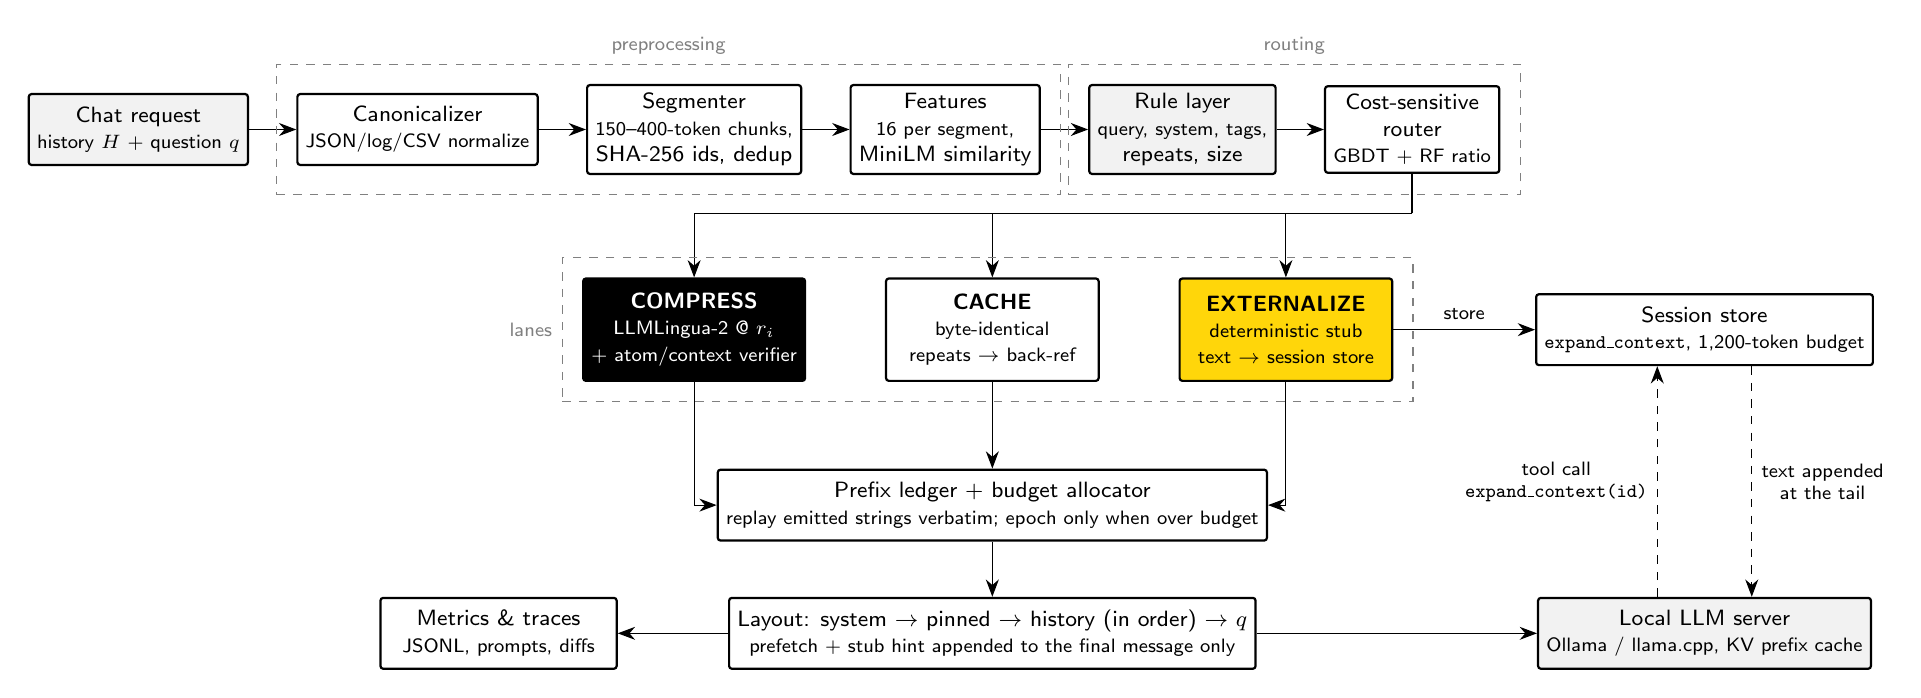
\begin{tikzpicture}[
  box/.style={draw, thick, rounded corners=1pt, font=\footnotesize\sffamily, align=center, minimum height=9mm, inner sep=3pt},
  lane/.style={box, minimum width=27mm, minimum height=13mm},
  lbl/.style={font=\scriptsize\sffamily, align=center},
  >={Stealth[length=2.2mm]}, node distance=6mm]
\node[box, fill=gray!10] (in) {Chat request\\{\scriptsize history $H$ + question $q$}};
\node[box, right=of in] (can) {Canonicalizer\\{\scriptsize JSON/log/CSV normalize}};
\node[box, right=of can] (seg) {Segmenter\\\scriptsize 150--400-token chunks,\\ SHA-256 ids, dedup};
\node[box, right=of seg] (feat) {Features\\\scriptsize 16 per segment,\\ MiniLM similarity};
\node[box, right=of feat, fill=gray!10] (rules) {Rule layer\\\scriptsize query, system, tags,\\ repeats, size};
\node[box, right=of rules] (clf) {Cost-sensitive\\router\\{\scriptsize GBDT + RF ratio}};
\node[lane, below=13mm of seg, fill=black, text=white] (c) {\textbf{COMPRESS}\\{\scriptsize LLMLingua-2 @ $r_i$}\\{\scriptsize + atom/context verifier}};
\node[lane, right=10mm of c, fill=white] (k) {\textbf{CACHE}\\{\scriptsize byte-identical}\\{\scriptsize repeats $\rightarrow$ back-ref}};
\node[lane, right=10mm of k, fill=lanegold] (x) {\textbf{EXTERNALIZE}\\{\scriptsize deterministic stub}\\{\scriptsize text $\rightarrow$ session store}};
\node[box, below=11mm of k, minimum width=60mm] (led) {Prefix ledger + budget allocator\\\scriptsize replay emitted strings verbatim; epoch only when over budget};
\node[box, below=7mm of led, minimum width=60mm] (lay) {Layout: system $\rightarrow$ pinned $\rightarrow$ history (in order) $\rightarrow$ $q$\\\scriptsize prefetch + stub hint appended to the final message only};
\node[box, minimum width=34mm] (store) [right=18mm of x] {Session store\\\scriptsize \texttt{expand\_context}, 1,200-token budget};
\node[box, fill=gray!10, minimum width=34mm] (srv) at (store |- lay) {Local LLM server\\\scriptsize Ollama / llama.cpp, KV prefix cache};
\node[box, left=14mm of lay, minimum width=30mm] (log) {Metrics \& traces\\\scriptsize JSONL, prompts, diffs};
\draw[->] (in)--(can); \draw[->] (can)--(seg); \draw[->] (seg)--(feat); \draw[->] (feat)--(rules); \draw[->] (rules)--(clf);
\coordinate (fork) at ($(clf.south)+(0,-5mm)$);
\draw[thick] (clf.south)--(fork);
\draw[->] (fork) -| (c.north); \draw[->] (fork) -| (k.north); \draw[->] (fork) -| (x.north);
\draw[->] (c.south) |- (led.west); \draw[->] (k.south)--(led.north); \draw[->] (x.south) |- (led.east);
\draw[->] (x.east)--node[lbl, above]{store}(store.west);
\draw[->] (led)--(lay); \draw[->] (lay)--(srv);
\draw[->, dashed] ($(srv.north)+(-6mm,0)$) -- node[lbl, left]{tool call\\\texttt{expand\_context(id)}} ($(store.south)+(-6mm,0)$);
\draw[->, dashed] ($(store.south)+(6mm,0)$) -- node[lbl, right]{text appended\\at the tail} ($(srv.north)+(6mm,0)$);
\draw[->] (lay)--(log);
\node[draw, dashed, gray, fit=(can)(seg)(feat), inner sep=2.5mm, label={[lbl, gray]above:preprocessing}] {};
\node[draw, dashed, gray, fit=(rules)(clf), inner sep=2.5mm, label={[lbl, gray]above:routing}] {};
\node[draw, dashed, gray, fit=(c)(k)(x), inner sep=2.5mm, label={[lbl, gray]left:lanes}] {};
\end{tikzpicture}}
\caption{Architecture of Sieve. Each segment takes exactly one lane. Rules run before the classifier and always win. The ledger
replays strings emitted on earlier turns byte-for-byte so the server's KV prefix stays valid; dashed edges show the tool round
trip that returns externalized text. All Sieve components run on the CPU.}\label{fig:arch}
\end{figure*}
Fig.~\ref{fig:arch} shows the pipeline. It is model-agnostic middleware between a chat client and an unmodified local server.

\subsection{Canonicalization, Segmentation and Features}
Tool output is first normalized losslessly where possible: JSON is minified, null and empty fields are dropped and identical records
collapsed with a count; consecutive identical log lines become one line with a multiplicity; duplicate CSV rows are counted. Each
message is then split on paragraph boundaries into chunks of 150--400 tokens. A segment's identifier is the first
12 hex digits of the SHA-256 of its text, so identical text always maps to the same identifier. Exact repeats are found by
identifier and near-duplicates by 5-word shingle Jaccard similarity $\ge 0.85$, both per session. Each segment receives 16
features: six core features (system flag, last-turn flag, normalized length, recency in turns, repeat count, and cosine similarity
to the current question computed with MiniLM~\cite{wang2020minilm} on the CPU), seven kind indicators, digit density,
near-duplicate score and prior expansion count.

\subsection{Rule Layer}
Rules are checked first, in priority order: (1) the current question is never altered; (2) the system prompt is cached; (3) user
tags are honored (\textit{never\_compress} and \textit{pinned} force CACHE; \textit{never\_externalize} forbids EXTERNALIZE); (4) an
exact repeat of an emitted segment becomes a one-line back-reference, and a near-duplicate does so only if every fact-like atom it
contains already appears in the original, so a changed value is never hidden; (5) segments under 40 tokens pass through;
(6) a segment whose stub would exceed half its size may not be externalized. Rules are user-extensible from configuration.

\subsection{Cost-Sensitive Router}
For the remaining segments a gradient-boosting classifier (150 trees, depth 3)~\cite{friedman2001gbm} estimates lane probabilities
$p\in\Delta^3$, trained with balanced sample weights~\cite{he2009imbalanced}. Sieve does not take the arg-max. It chooses
\begin{equation}
\hat\ell=\arg\min_{j}\sum_{i} p_i\,C_{ij},\qquad C_{\textsc{c},\textsc{x}}=5,\ C_{ij}=1\ (i\ne j),\ C_{ii}=0,
\label{eq:cost}
\end{equation}
so hiding a segment that should have been sent costs 5 times more than any other mistake. If $\max_i p_i<0.55$
the segment falls back to COMPRESS at $r=0.9$, never to EXTERNALIZE. A random forest~\cite{breiman2001rf} predicts the keep-ratio
of COMPRESS segments; the prediction is snapped to $\mathcal{R}$ and floored per kind (documents 0.3, chat 0.4, instructions 0.9).

\subsection{COMPRESS Lane and Fact Verifier}
Compression uses LLMLingua-2~\cite{pan2024llmlingua2} on the CPU. Results are memoized on (content hash, ratio, compressor
version), so the same input always produces the same string. Before compression, the verifier extracts atoms $A$: numbers, dates,
versions, identifiers, quoted strings and capitalized entities. After compression it computes
\begin{equation}
\mathrm{AR}=\frac{|\{a\in A: a\ \text{in output}\}|}{|A|},\qquad
\mathrm{CR}=\min_{a\in A}\frac{|W_a\cap N_a|}{|W_a|},
\label{eq:verify}
\end{equation}
where $W_a$ is the set of content words of the sentence containing $a$ (excluding atom words) and $N_a$ the words within $\pm12$
positions of $a$ in the output. Compression is accepted if every numeric or identifier atom survives, $\mathrm{AR}\ge0.9$ and
$\mathrm{CR}\ge0.5$; otherwise the ratio is raised one bucket, up to 3 times, and finally the segment passes through
uncompressed. The context-recall term was added after LLMLingua-2 was observed to keep a person's name while deleting the role
that made it an answer; atom recall alone did not catch this. A repair step undoes tokenizer artifacts of the compressor (for
example ``5 585'' $\rightarrow$ ``5,585'') for atoms present in the original text only.

\subsection{CACHE and EXTERNALIZE Lanes}
CACHE emits the segment unchanged. EXTERNALIZE stores the full text in a session-scoped dictionary and emits a deterministic stub
\texttt{[ref:ID | kind | Nt | "summary" | keys: \dots{} | use expand\_context("ID")]}, whose summary is extractive (leading sentence
plus top TF-IDF terms) and whose keys are up to five salient atoms. When all chunks of a message are externalized they share one
stub. The model can call \texttt{expand\_context} (at most 2 rounds per request, 1,200 tokens per request); unknown
identifiers return an explicit error rather than empty text, so the model cannot be misled into inventing content. With reasoning
disabled, the model rarely called the tool on its own, so Sieve appends one line to the final user message listing up to six stub
identifiers with their keys. Prefetching expands stubs whose similarity to the question is at least 0.75. Both the hint
and prefetched text sit in the final message, after the cached prefix.

\subsection{Prefix Ledger and Epochs}
\begin{algorithm}[t]\caption{Per-turn prompt assembly with the prefix ledger}\label{alg:turn}\small
\begin{algorithmic}[1]
\Require history $H$, question $q$, ledger $\mathcal{L}$ (segment key $\mapsto$ emitted string), store $S$
\State $G\gets\textsc{Segment}(H\cup\{q\})$; compute features of $G$ w.r.t.\ $q$
\If{$\mathcal{L}=\emptyset$} \State $E\gets\textsc{RouteAll}(G)$; $\textit{epoch}\gets$ true
\Else
  \State $E\gets\{g\mapsto\mathcal{L}[g]: g\in G\cap\mathcal{L}\}$ \Comment{replay verbatim}
  \State $E\gets E\cup\textsc{Route}(G\setminus\mathcal{L})$
  \If{$|E|+\text{hint}+R>0.8\,n_\text{ctx}$} \State $E\gets\textsc{RouteAll}(G)$; $\textit{epoch}\gets$ true \EndIf
\EndIf
\If{\textit{epoch} and $|E|+\text{hint}+R>0.8\,n_\text{ctx}$} \State $E\gets\textsc{Allocate}(E,\ 0.85\cdot(0.8\,n_\text{ctx}-R))$ \EndIf
\State $P\gets\textsc{Layout}(E)$ $+$ prefetch $+$ stub hint \Comment{tail only}
\State $\mathcal{L}\gets E$; \Return $P$
\end{algorithmic}\end{algorithm}
The ledger stores the exact string emitted for every segment (Algorithm~\ref{alg:turn}). On later turns it replays those strings
and routes only new segments, so the prompt grows by appending and the cached prefix remains valid. Old segments are not re-scored,
even though their similarity to the new question has changed. A full re-route, an \emph{epoch}, happens only when the projected
prompt plus the output reserve would exceed 80\% of $n_\text{ctx}$; the allocator then targets 85\% of that
threshold so that the next turns do not immediately trigger another epoch. The tool definition is attached the first time anything is
externalized and then kept, because the server renders tools inside the system block and toggling them would invalidate the whole
prefix.

\subsection{Budget Allocator}\label{sec:budget}
\begin{algorithm}[t]\caption{Greedy budget allocation}\label{alg:alloc}\small
\begin{algorithmic}[1]
\Require emitted segments $E$, target $\tau$, hard limit $B$
\State $Q\gets$ unprotected segments sorted by (similarity to $q$, turn, position) ascending
\For{$s\in Q$ \textbf{while} $|E|>\tau$} lower $r_s$ to its kind floor; recompress and verify \EndFor
\For{$s\in Q$ \textbf{while} $|E|>\tau$} \If{EXTERNALIZE allowed for $s$} externalize $s$ \EndIf \EndFor
\For{$s\in Q$ by age \textbf{while} $|E|>B$} drop $s$; flag hard truncation \EndFor
\end{algorithmic}\end{algorithm}
Algorithm~\ref{alg:alloc} tightens the least relevant and oldest segments first: it lowers ratios, then externalizes, and drops
segments only as a last resort, which is logged as a hard truncation. Protected segments (question, system prompt, pinned and
\textit{never\_compress} text, back-references) are never touched. After allocation the prompt is rendered and counted exactly; if
it still exceeds $B$, allocation repeats against the exact count.

\subsection{Complexity}
For a request with $n$ tokens in $m$ segments: canonicalization, tokenization and chunking are $O(n)$; exact-duplicate detection is
$O(m)$ with a hash map; near-duplicate detection compares shingle sets pairwise, $O(m^2 k)$ for $k$ shingles per segment; features
cost $O(m)$ encoder passes of bounded length; rule checks are $O(m)$; routing is $O(m\,T\,d)$ for $T$ trees of depth $d$; ledger
replay is $O(m)$ dictionary lookups; and the allocator sorts once, $O(m\log m)$, then makes at most two linear passes, each step
re-compressing one segment of at most 400 tokens. Compression and embedding results are memoized, so a replayed turn costs
only the new segments. Measured CPU overhead is reported in Section~\ref{sec:results}.

%=====================================================================
\section{Experimental Methodology}\label{sec:exp}
\subsection{Research Questions}
\begin{itemize}
\item \textbf{RQ1} Does Sieve reduce prompt tokens and increase output headroom without lowering accuracy?
\item \textbf{RQ2} How does it affect time to first token on cold and warm questions?
\item \textbf{RQ3} Does compression invalidate the server's prefix cache, and does the ledger prevent it?
\item \textbf{RQ4} Which components matter (verifier, ledger, router, prefetch)?
\item \textbf{RQ5} How accurate is the router on conversations it has not seen, and when does externalization stop paying off?
\end{itemize}

\subsection{Platform}
All runs used Qwen3-14B~\cite{qwen3} at Q4\_K\_M quantization (14.8B parameters) served by Ollama 0.32.15~\cite{ollama}
on an Apple M5 Pro with 24\,GB of unified memory; the server reported the model fully resident on the GPU (100\% of
8.97\,GiB). Requests used $n_\text{ctx}=4096$, at most 64 output tokens, temperature 0, a fixed seed and
reasoning disabled; the selfcheck confirmed that no reasoning tokens were produced. Sieve's components (LLMLingua-2 BERT-base,
MiniLM, scikit-learn~\cite{pedregosa2011sklearn}) ran on the CPU. Token totals use the Qwen tokenizer with a chat-template overhead
calibrated against the server; on a 1,821-token calibration prompt the tokenizer and the server agreed exactly
(1,821 vs.\ 1,821).

\subsection{Workload Generation}
Conversations are generated from seed 7 with invented entities (codenames, people, figures), so the model cannot answer from
prior knowledge. Filler text comes from a template grammar that contains no digits and no invented names; a unit test checks that
each gold value appears only in the messages that the ground truth marks as needed. The benchmark has 76 conversations with
180 evaluation questions in eleven families (Table~\ref{tab:fam}). After each question is answered, the scripted gold answer is
appended to the history, so a wrong answer never propagates and every condition sees the same history. Question types are
numeric lookup (67), name lookup (64), decision recall (20), multi-hop (9), unanswerable (8), latest-value tracking (8), negation (4). 26\% of questions (47 of 180) had a raw prompt longer than $n_\text{ctx}$. The router was
trained on 456 further conversations from six seeds disjoint from the benchmark seed.
\begin{table}[t]\centering\caption{Workload families (questions per family in parentheses).}\label{tab:fam}\footnotesize
\begin{tabular}{cl}\toprule ID & What the family stresses\\\midrule
A & Long system prompt, short chat (19)\\
B & Long chat, old irrelevant history (20)\\
C & Verbose document Q\&A (27)\\
D & Same document re-pasted (18)\\
E & Needle in a haystack (10)\\
F & Topic switches, late recall (16)\\
G & Number / ID dense text (16)\\
H & Bloated tool output (6)\\
I & Code Q\&A (8)\\
J & Adversarial edge cases (8)\\
K & Mixed 10–20 turn sessions (32)\\
\bottomrule\end{tabular}\end{table}

\subsection{Conditions}
Table~\ref{tab:cond} lists the conditions. C1 and C2 are matched per question to the prompt size C4 produced, so they compare
strategies at an equal token budget. The five ablations each remove or replace one component of C4.
\begin{table}[t]\centering\caption{Experimental conditions.}\label{tab:cond}\footnotesize\setlength{\tabcolsep}{3pt}
\begin{tabular}{lp{0.70\columnwidth}}\toprule
C0 & Raw prompt (baseline), append-only history.\\
C1 & Truncation: drop oldest whole messages to C4's token count.\\
C2 & One uniform LLMLingua-2 rate on all unprotected segments, matched to C4's token count.\\
C3 & Sieve with rules and the hand-written heuristic labeller; no classifier, no verifier.\\
C4 & Full Sieve: rules, classifier, ledger/epochs, verifier, tools and prefetch.\\
C5 & C4 without ledger or memo: re-routes and re-compresses every turn.\\
C6 & Raw prompt with $n_\text{ctx}=8192$: accuracy reference.\\\midrule
Ablations & C4 $-$verifier; C4 $-$prefetch (tool only); C4 $-$ledger; C4 with a heuristic-trained classifier; C4 with only the six core features.\\
\bottomrule\end{tabular}\end{table}

\subsection{Protocol}
Each condition ran as its own operating-system process and its own pass over all conversations; conditions were never interleaved,
so no condition could inherit another's cache. The model was unloaded and reloaded before each pass. The first question of every
conversation is \emph{cold}, a novel prompt after a fresh load; later questions are \emph{warm}. Each of the 2,160 model
calls was logged with its prompt, response, per-segment decision trace and prompt diff.

\subsection{Metrics and How They Are Derived}
Table~\ref{tab:metrics} defines every reported quantity and the logged field it is computed from.
\begin{table}[t]\centering\caption{Metric definitions. $T_\text{raw}$, $T_\text{sent}$: tokenizer counts of the raw and the sent
prompt, including chat template and all Sieve overhead.}\label{tab:metrics}\scriptsize\setlength{\tabcolsep}{2.5pt}
\begin{tabular}{lp{0.66\columnwidth}}\toprule
Accuracy & Mean of a per-question score: normalized containment of a gold string; exact integer match for numbers; day, month and year all present for dates; first yes/no word; refusal pattern without numbers for unanswerable questions.\\
Tokens saved & $1-T_\text{sent}/T_\text{raw}$, paired per question with C0.\\
Headroom & $n_\text{ctx}-T_\text{sent}$.\\
TTFT & Client time from sending the request to the first answer token, including tool round trips.\\
Prefix reuse & $1-t_\text{prefill}/\hat t_\text{cold}(T_\text{sent})$, with $\hat t_\text{cold}(n)=an+bn^2$ fitted on novel prompts (Sec.~\ref{sec:reuse}).\\
Prefilled tokens & $T_\text{sent}\times(1-\text{reuse})$, summed over a conversation.\\
Atom recall & Share of the question's gold atoms present in the sent prompt.\\
Sieve CPU & Segmentation, routing, compression, verification and assembly time per call.\\
Decode speed & Generated tokens / generation time; independent of the prompt, used as a machine-health indicator.\\
\bottomrule\end{tabular}\end{table}

\subsection{Statistical Analysis}
Every comparison is paired by question against C0. For a statistic $\theta$ of the per-question differences we report the observed
value and a 95\% percentile bootstrap interval from 2,000 resamples of questions~\cite{efron1979bootstrap}; medians are used for
latency. A difference is called significant only when its interval excludes zero. The claims list is generated by the same code.

\subsection{Measuring Prefix Reuse}\label{sec:reuse}
On this server the reported \texttt{prompt\_eval\_count} equals the full prompt length even when the prefix comes from the cache,
so it cannot reveal reuse. Prefill \emph{time}, however, collapses on a cache hit. We therefore fit cold prefill time on novel
prompts of 286, 545, 1,058, 1,841, 2,648, 3,435 tokens, obtaining $a=1.699$\,ms per token and $b=0.0419$\,\textmu s per token$^2$, and estimate reuse as in
Table~\ref{tab:metrics}. Section~\ref{sec:rq3} validates the estimator.

\subsection{Data Integrity Safeguards}
Three issues arose during the campaign and were handled as follows. (i) A first full run was discarded after the host began swapping
memory, which depressed decode speed; every call now carries a flag when decode speed falls below half the calibrated value.
(ii) During a network outage three passes silently fell back to an approximate tokenizer and, for two of them, to an extractive
compressor; they were discarded and rerun with models loaded offline, and the benchmark now refuses to run with any degraded
component. All 2,160 analysed calls ran with the exact tokenizer and LLMLingua-2 (0 fallbacks). (iii) One
conversation of one pass was interrupted and re-run; the analysis keeps the last record per question. Residual machine-load
variation is reported in Section~\ref{sec:rq2}.

%=====================================================================
\section{Results}\label{sec:results}
\begin{table*}[t]\centering
\caption{Results per condition over 180 questions from 76 conversations. Accuracy with 95\% bootstrap interval. Prompt
tokens are those actually sent, including all Sieve overhead. TTFT medians in seconds. Reuse is the timing-derived share of prefill
skipped. Decode is the pass's median decode speed (machine-health indicator).}\label{tab:main}
\resizebox{\textwidth}{!}{%
\begin{tabular}{lcrrrrrrrr}\toprule
Condition & Accuracy [95\% CI] & Prompt tok. & Saved\,\% & Headroom & TTFT$_\text{cold}$ & TTFT$_\text{warm}$ & Reuse\,\% & Sieve CPU (ms) & Decode (tok/s)\\\midrule
C0 Raw prompt & 0.861 [0.81, 0.91] & 2,747 & 0.0 & 1,349 & 3.26 & 0.46 & 47 & 0 & 26.8\\
C1 Truncate & 0.444 [0.37, 0.52] & 999 & 58.7 & 3,097 & 0.48 & 0.42 & 17 & 0 & 27.4\\
C2 Uniform LLMLingua-2 & 0.778 [0.72, 0.84] & 1,652 & 33.6 & 2,444 & 3.19 & 0.43 & 34 & 957 & 17.4\\
C3 Sieve, rules & 0.878 [0.83, 0.92] & 1,646 & 34.7 & 2,450 & 2.64 & 0.42 & 44 & 69 & 28.7\\
C4 Sieve, full & 0.911 [0.87, 0.95] & 1,703 & 31.0 & 2,393 & 2.50 & 0.33 & 45 & 84 & 28.9\\
C5 Sieve, no ledger & 0.917 [0.87, 0.96] & 1,698 & 30.9 & 2,398 & 3.41 & 3.49 & 13 & 2,022 & 15.6\\
C6 8k context & 0.994 [0.98, 1.00] & 2,747 & 0.0 & 5,445 & 7.14 & 0.75 & 39 & 0 & 15.4\\
\bottomrule\end{tabular}}\end{table*}

\begin{table}[t]\centering
\caption{Paired differences against C0: mean [95\% bootstrap CI]. The last column covers the 47 questions whose raw prompt
exceeded $n_\text{ctx}$.}\label{tab:paired}
\resizebox{\columnwidth}{!}{%
\begin{tabular}{lcccc}\toprule
 & $\Delta$Acc (pp) & Saved (\%) & $\Delta$TTFT$_\text{cold}$ (s) & $\Delta$Acc, overflow (pp)\\\midrule
C1 & -41.7 [-48.9, -34.4] & 58.7 [53.4, 63.6] & -1.36 [-2.32, -0.58] & -8.5 [-17.0, -2.1]\\
C2 & -8.3 [-13.9, -2.8] & 33.6 [30.4, 36.5] & -0.25 [-0.61, 0.05] & -4.3 [-19.2, 12.8]\\
C3 & +1.7 [-5.0, 7.8] & 34.7 [31.5, 37.5] & -1.15 [-1.47, -0.92] & +36.2 [21.3, 51.1]\\
C4 & +5.0 [-0.6, 11.1] & 31.0 [27.8, 34.0] & -1.12 [-1.49, -0.66] & +36.2 [19.1, 53.2]\\
C5 & +5.6 [0.0, 11.1] & 30.9 [27.5, 33.9] & -0.20 [-0.38, 0.15] & +34.0 [17.0, 51.1]\\
C6 & +13.3 [8.3, 18.3] & 0.0 [0.0, 0.0] & +2.14 [1.61, 2.80] & +51.1 [36.2, 66.0]\\
\bottomrule\end{tabular}}\end{table}

\subsection{RQ1: Tokens, Headroom and Accuracy}
Tables~\ref{tab:main} and~\ref{tab:paired} answer RQ1. C4 sent 1,703 prompt tokens on average against 2,747 for C0, a paired
reduction of 31.0\% (95\% CI 27.8--34.0\%), and mean output headroom rose from 1,349 to 2,393 tokens. Accuracy was
0.911 for C4 and 0.861 for C0; the paired difference of +5.0 percentage points (CI -0.6 to +11.1) is not statistically distinguishable from zero. The gain is concentrated where the raw prompt overflowed the window and the server truncated it: on those 47 questions C4 changed accuracy by +36.2 pp (CI +19.1 to +53.2). The 8k-context reference C6 reached 0.994, which bounds what any
prompt-shaping method can recover here. At a matched budget, truncation (C1) changed accuracy by -41.7 pp (CI -48.9 to -34.4)
because it drops whole documents, and uniform compression (C2) by -8.3 pp (CI -13.9 to -2.8). Fig.~\ref{fig:trade} plots savings
against accuracy for every condition.
\begin{figure}[t]\centering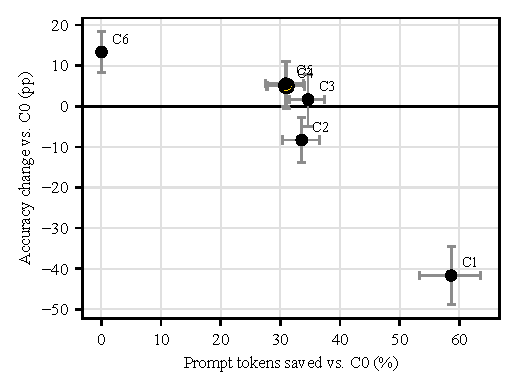
\includegraphics[width=\columnwidth]{fig_tradeoff.pdf}
\caption{Prompt-token savings versus accuracy change relative to C0, with 95\% paired bootstrap intervals. C4 is the filled yellow
marker. Derived from the paired per-question differences in the run log.}\label{fig:trade}\end{figure}

\subsection{RQ2: Latency}\label{sec:rq2}
\begin{figure}[t]\centering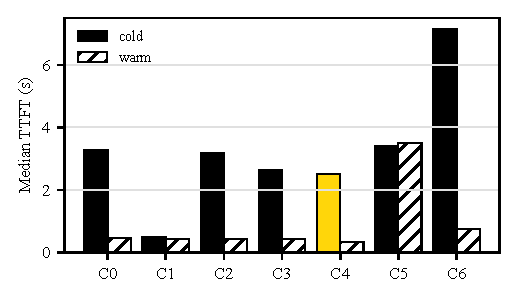
\includegraphics[width=\columnwidth]{fig_ttft.pdf}
\caption{Median time to first token for cold (first question of a conversation) and warm (later) questions per condition.}\label{fig:ttft}\end{figure}
On cold questions C4 reduced median TTFT by 1.12 s (CI 0.66 to 1.49), because it prefills fewer tokens (Fig.~\ref{fig:ttft}). On warm questions most of the raw prompt is already cached and the medians were 0.33 s for C4 and
0.46 s for C0. Mean Sieve CPU time was 84 ms per call for C4. Decode speed does not depend on the prompt, so it serves as a health indicator for the host. The passes C2 Uniform LLMLingua-2, C5 Sieve, no ledger, C6 8k context, C4 $-$verifier ran at a median decode speed below 75\% of C0's 26.8 tok/s because of host memory pressure (calls flagged as degraded: C2 18, C5 11, C6 35, C4 16). Their absolute latencies are inflated and are not used for latency comparisons; their token and accuracy results are unaffected. C0 and C4 ran at matching decode speeds (26.8 and 28.9 tok/s).

\subsection{RQ3: The Cache--Compression Conflict}\label{sec:rq3}
\begin{figure}[t]\centering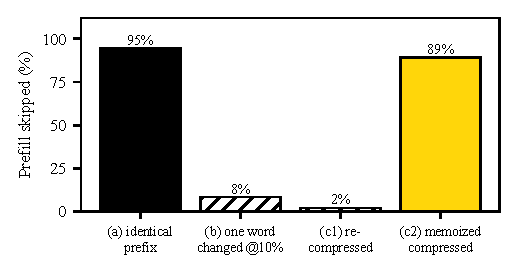
\includegraphics[width=\columnwidth]{fig_cachetest.pdf}
\caption{Controlled cache test on the live server: share of the second request's prefill that the server skipped.}\label{fig:ct}\end{figure}
Fig.~\ref{fig:ct} isolates the conflict with four request pairs on a 1,871-token prefix. With an identical prefix the server
skipped 95\% of prefill; changing a single word at 10\% depth reduced reuse to 8\%, close to the 10\% that precedes the
change, which validates the timing estimator. Re-compressing the prefix at a different ratio reduced reuse to 2\%, and sending
the memoized compressed string restored it to 89\%. The benchmark shows the same effect at scale: C4 averaged 45\% prefix
reuse with 84 ms of CPU per call, while C5, which re-routes and re-compresses every turn, averaged 13\% reuse and
2,022 ms of CPU per call. Summed over a conversation, C4 prefilled 1,981 tokens, C5 3,268 and C0 2,824.

\subsection{RQ4: Ablations}
\begin{table}[t]\centering\caption{Ablations of C4 over 180 questions. Prefill/conv.: tokens prefilled per conversation.}\label{tab:abl}
\resizebox{\columnwidth}{!}{%
\begin{tabular}{lrrrrrr}\toprule
Variant & Acc. & $\Delta$Acc vs C0 (pp) & Saved\,\% & Reuse\,\% & Prefill/conv. & Re-infl.\\\midrule
C4 Sieve, full & 0.911 & +5.0 [-0.6, 11.1] & 31.0 & 45 & 1,981 & 270\\
C4 $-$verifier & 0.850 & -1.1 [-7.8, 5.6] & 32.6 & 41 & 2,102 & 0\\
C4 $-$prefetch & 0.911 & +5.0 [-0.6, 11.1] & 31.0 & 42 & 2,118 & 270\\
C4 $-$ledger & 0.917 & +5.6 [0.0, 11.1] & 30.9 & 17 & 3,064 & 373\\
C4, heuristic-trained & 0.917 & +5.6 [0.0, 11.7] & 32.6 & 43 & 2,049 & 268\\
C4, core-6 features & 0.939 & +7.8 [2.8, 13.3] & 31.2 & 44 & 2,059 & 255\\
\bottomrule\end{tabular}}\end{table}
Table~\ref{tab:abl} removes one component at a time. Removing the verifier changed accuracy from 0.911 to 0.850 while saving 32.6\% of tokens instead of 31.0\%; with the verifier, C4 re-inflated 270 segment compressions. Removing the ledger lowered mean prefix reuse from 45\% to 17\% and raised prefill per conversation from 1,981 to 3,064 tokens. The classifier trained on heuristic labels reached 0.917 and the classifier restricted to the six core features 0.939, against 0.911 for C4; their paired intervals overlap with C4's. Prefetching never triggered in any condition, so the $-$prefetch variant sent the same prompts as C4.

\subsection{RQ5: Router Accuracy and Externalization Break-Even}
\begin{table}[t]\centering\caption{Routers on held-out conversations (14,586 segment decisions from 456 conversations,
GroupKFold by conversation; ground truth = oracle labels). Dangerous: a segment needed by a current or future question sent to
EXTERNALIZE (out of 1,897).}\label{tab:clf}
\resizebox{\columnwidth}{!}{%
\begin{tabular}{lrcrr}\toprule Router & Macro-F1 & Ext.\ P / R & Ratio MAE & Dangerous\\\midrule
Hard rules only & 0.642 & 0.00 / 0.00 & 0.367 & 0\\
Heuristic labeller (C3) & 0.912 & 0.73 / 0.85 & 0.052 & 147\\
GBDT, heuristic labels & 0.910 & 0.73 / 0.85 & 0.055 & 146\\
GBDT, oracle labels (C4) & 0.949 & 0.94 / 0.83 & 0.023 & 79\\
GBDT, oracle, core-6 & 0.943 & 0.90 / 0.84 & 0.044 & 137\\
\bottomrule\end{tabular}}\end{table}
Table~\ref{tab:clf} scores the routers on conversations they never saw. The oracle-trained classifier reached macro-F1 0.949 with
79 dangerous errors, against 147 for the heuristic labeller; inference took 0.007 ms per segment. Because the
oracle label is partly a fixed function of the features (age, size and repetition), a high F1 mainly shows that the labelling rule is
learnable; the downstream comparison of C3 and C4 (Table~\ref{tab:main}) is the more meaningful evidence.
Fig.~\ref{fig:be} sweeps the probability $p$ that a question needs a large archived document that C4 externalizes (8 cold conversations per point). Mean net time per question was 4.47 s for C4 and 8.51 s for C0 at $p=0$, and 7.63 s and 9.42 s at $p=1$, where C4 expanded on 75\% of questions. The curves did not cross in the swept range: in this setting externalization paid off even when every question needed the document, because C0's prompt overflowed the window and was prefilled in full on every call. Accuracy at $p=1$ was 0.88 for C4 and 0.50 for C0.
\begin{figure}[t]\centering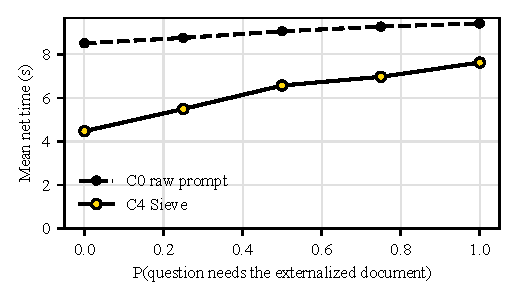
\includegraphics[width=\columnwidth]{fig_breakeven.pdf}\caption{Externalization break-even: mean net time per question (Sieve CPU time plus model time, including tool round trips) as the probability that a question needs the externalized document grows.}\label{fig:be}\end{figure}

\subsection{Breakdown by Workload}
\begin{table}[t]\centering\caption{Accuracy by workload family (bold: above C0 on the same questions).}\label{tab:famres}
\resizebox{\columnwidth}{!}{%
\begin{tabular}{lrrrrrrrr}\toprule Fam. & $n$ & C0 & C1 & C2 & C3 & C4 & C5 & C6\\\midrule
A & 19 & 0.84 & 0.84 & 0.84 & 0.84 & 0.84 & 0.84 & \textbf{1.00}\\
B & 20 & 0.90 & 0.65 & 0.90 & \textbf{1.00} & \textbf{1.00} & \textbf{0.95} & \textbf{0.95}\\
C & 27 & 0.74 & 0.00 & \textbf{0.78} & \textbf{0.81} & \textbf{1.00} & \textbf{1.00} & \textbf{1.00}\\
D & 18 & 1.00 & 0.17 & 0.56 & 0.89 & 0.78 & 1.00 & 1.00\\
E & 10 & 0.80 & 0.20 & 0.70 & \textbf{0.90} & \textbf{1.00} & \textbf{1.00} & \textbf{1.00}\\
F & 16 & 0.94 & 0.50 & 0.81 & 0.94 & \textbf{1.00} & \textbf{1.00} & \textbf{1.00}\\
G & 16 & 0.62 & 0.00 & 0.62 & \textbf{0.94} & \textbf{0.88} & \textbf{0.88} & \textbf{1.00}\\
H & 6 & 0.83 & 0.00 & 0.67 & \textbf{1.00} & 0.83 & 0.83 & \textbf{1.00}\\
I & 8 & 0.75 & 0.50 & \textbf{0.88} & 0.50 & 0.75 & 0.62 & \textbf{1.00}\\
J & 8 & 0.88 & 0.88 & 0.88 & 0.62 & 0.75 & 0.88 & \textbf{1.00}\\
K & 32 & 1.00 & 0.84 & 0.84 & 0.94 & 0.94 & 0.88 & 1.00\\
\bottomrule\end{tabular}}\end{table}
Table~\ref{tab:famres} breaks accuracy down by family. Groups are small, so single rows are indicative only. C4 was above C0 in families B, C, E, F, G and below it in D, J, K.

%=====================================================================
\section{Discussion}\label{sec:discussion}
\textit{What the results support.} Sieve reduced prompt tokens by 31.0\% with an interval that excludes zero, improved accuracy on prompts that overflowed the window (+36.2 pp), lowered median cold TTFT by 1.12 s; its overall accuracy change is not statistically distinguishable from zero. The cache test and the C4--C5 comparison support the ledger as the mechanism that keeps compression compatible with prefix caching.

\textit{Where Sieve does not help.} On short prompts (under about 1,500 tokens) C4 saved 15.8\% of tokens and reached accuracy 0.94 against 1.00 for C0. Families D, J, K lost accuracy under C4. On warm questions the raw prompt's prefix is already cached, so latency differences there are small (0.33 s vs.\ 0.46 s median). C4 hard-truncated 15 prompts that remained over budget after compression and externalization.

\textit{Tool use without reasoning.} With reasoning disabled, the model called \texttt{expand\_context} only when prompted by the
tail hint; C4 expanded on 5\% of questions, and 4 needed segments were stubbed but never expanded. Prefetching never triggered at the 0.75 similarity threshold, so the $-$prefetch ablation sent the same content as C4 and differs only in timing.

\textit{Threats to validity.} \emph{Internal:} latency depends on machine state; we ran conditions in separate passes, flagged slow
calls and report decode speed per pass. \emph{Construct:} prefix reuse is estimated from a fitted cold-prefill curve rather than read
from the server. \emph{External:} the workloads are synthetic with invented entities, the benchmark is small, and it covers one model
on one machine with no CPU offload; results describe this suite rather than real conversations. Stub summaries are extractive and
only text attachments are supported.

%=====================================================================
\section{Conclusion}\label{sec:conclusion}
Sieve routes each segment of a prompt to compression, caching or externalization and keeps the emitted text byte-stable with a
ledger. On 180 ground-truth questions with Qwen3-14B and a 4096-token window, it reduced prompt tokens by 31.0\%
and raised output headroom from 1,349 to 2,393 tokens, with accuracy statistically indistinguishable from the raw prompt; on questions whose raw prompt overflowed the window, accuracy rose by 36.2 percentage points A controlled test showed that re-compressing a
prefix destroys prefix reuse and that byte-stable memoized output restores it. Future work includes evaluating real conversation
logs, other model families and servers, abstractive stub summaries, and learning when to expand rather than prompting for it.

\section*{Code and Data Availability}
The implementation, configuration, benchmark generator, test suite, all 2,160 logged calls with per-segment traces, and the
scripts that regenerate every table and figure in this paper are available at \url{https://github.com/Tarun-Vaibhav-V/sieve}~\cite{sieve2026code}.

\bibliographystyle{IEEEtran}
\bibliography{refs}

\begin{IEEEbiographynophoto}{[Author Name]}
[Short biography: degree, institution, research interests.]
\end{IEEEbiographynophoto}
\end{document}
